\documentclass[a4paper]{article}
\usepackage{tikz}
\usepackage{amsmath}
\usepackage{mathtools}
\usepackage{hyperref}
\usepackage{tikz}
\usetikzlibrary{patterns,arrows.meta}
\begin{document} 

\section{AULA 1}

\subsection{Lei de Coulomb}
\begin{center}
    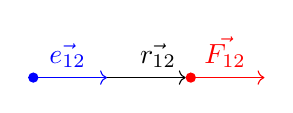
\begin{tikzpicture}
        \draw[->] (0,0) -- (2,0) node[above left] {$ \vec{r_{12}} $};
        \draw[red,Circle->](2,0) -- (3,0) node[midway,above] {$ \vec{F_{12}} $};
        \draw[blue, Circle->] (0,0) -- (1,0)node[midway,above] {$ \vec{e_{12}} $};
        \end{tikzpicture}
\end{center}

A força entre duas cargas pontuais $q_{1}$ e $q_{2}$ é dada por
\[ \vec{F}_{12} = K_e \frac{q_1 q_2}{r_{12}^2} \vec{e_{r_{12}}}\] 
onde 
\[K_e=\frac{1}{4\pi\epsilon_0} \]
\[ K_e =9*10^9 NC^{-2}m^{-2} \]
\[ \epsilon_0 = \frac{1}{4\pi*9*10^9} 
= 8.85*10^{-12} N^{-1}C^2m^{-2}\]
$\epsilon_0$ é conhecida como a permitividade do vácuo


\subsection{Forca Elétrica vs Força Gravítica}
\[F_g = G \frac{m_1m_2}{r^2},     F_e = K_e \frac{q_1 q_2}{r_{12}^2}\]
A força entre dois protões afastados por uma distância d
\[\frac{F_e}{F_g}= \frac{9*10^9 \frac{{(1.6*10^{-19})}^2}{d^2}}{6.7*10^{-11} \frac{{(1.7*10^{-27})}^2}{d^2}} = 10^{36}\] 
Isto é, a interação elétrica entre os dois protões é $10^{36}$
 vezes maior que a interação gravítica entre eles
,logo para partículas carregadas a interação gravítica é desprezável

\subsection{Campo Elétrico}
O campo elétrico ($\vec{E}$) é a força por unidade de carga através do 
efeito de uma carga q sobre o espaço á sua volta.
Este é dado pela divisão da lei de coulomb por $q_2$.
\begin{center}
    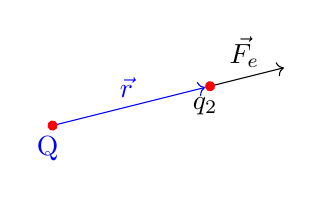
\begin{tikzpicture}
        \draw [blue,{Circle[red]}->] (0,0)--(2,0.5) node[midway,above] {$ \vec{r} $} node[at start,below] {Q};
        \draw [black,{Circle[red]}->] (2,0.5)--(3,0.75) node[midway,above] {$ \vec{F_e}$} node[at start,below] {$q_2$};
    \end{tikzpicture}
\end{center}
\[\vec{E} = \frac{\vec{F_e}}{q} = \frac{1}{4\pi\epsilon_0} \frac{Q}{r^2}\vec{e_r}\]
\[\vec{F}= q\vec{E}\]

\subsection{Principio de Sobreposição}
A força total das forças aplicadas numa carga é igual a soma vetorial 
de todas as forças que lhe são aplicadas por outras partículas
\begin{center}
    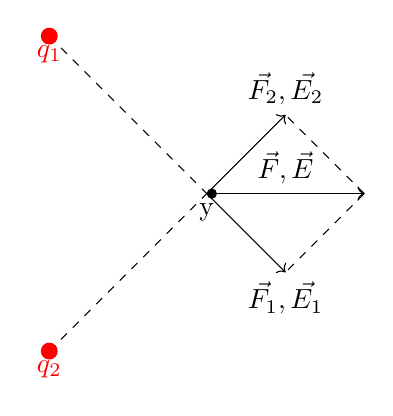
\begin{tikzpicture}
        \draw [black,{Circle[]}->] (0,0)--(2,0) node[at start,below] {y} node[midway,above] {$ \vec{F},\vec{E}$};
        \draw [black,->] (0,0)--(1,-1) node[below] {$ \vec{F_1},\vec{E_1}$};
        \draw [black,->] (0,0)--(1,1)  node[above] {$ \vec{F_2},\vec{E_2}$};
        \draw [black,dashed] (2,0)--(1,-1);
        \draw [black,dashed] (2,0)--(1,1) ;
        \draw [black,dashed] (-2,2)--(0,0);
        \draw [black,dashed] (-2,-2)--(0,0);
        \draw [red,fill=red](-2,2) circle [radius=0.1] node [below] {$q_1$};
        \draw [red,fill=red](-2,-2) circle [radius=0.1]node [below] {$q_2$};
    \end{tikzpicture}
\end{center}
\[ \vec{E} = \sum_{i}^{}\vec{E_i} 
= \sum_{i}^{} \frac{1}{4\pi\epsilon_0} \frac{q_i}{r_i^2} \vec{e_{r_i}} \]

\subsection{Distribuição Contínua de Carga}
As cargas são discretas, mas num corpo carregado as suas distâncias são tão pequenas que não as conseguimos distinguir umas das outras.
É então util passar a tratar essas cargas como uma distribuição contínua

\subsubsection{Ao Longo de uma linha (1D)}
A distribuição da carga é representada por $\lambda$[C/m] medido em coulombs por metro
\[dq = \lambda dl\]

\subsubsection{Numa Superfície (2D)}
A distribuição da carga é representada por G[C/m²] medido em coulombs por metro quadrado
\[dq = Gds\]

\subsubsection{Num Volume (3D)}
A distribuição da carga é representada por $\rho$ [C/m³] medido em coulombs por metro cúbico
\[dq = \rho dv\]


O campo elétrico criado por cada dq, sendo dq pontual é dado por:
\[d\vec{E} = \frac{1}{4\pi\epsilon_0} \frac{dq}{r^2} \vec{e_r}\]
e aplicando o principio da sobreposição,
\[\vec{E}= \int_{objeto}{d\vec{E}}\]
concretizando-se para cada um dos casos
\[1D:        \vec{E} = \frac{1}{4\pi\epsilon_0} \int_{\Gamma}{\frac{\lambda dl}{r^2}} \]
\[2D:        \vec{E} = \frac{1}{4\pi\epsilon_0} \int_{S}{\frac{Gdl}{r^2}} \]
\[3D:        \vec{E} = \frac{1}{4\pi\epsilon_0} \int_{v}{\frac{\rho dl}{r^2}} \]

\subsection{Trabalho Do Campo Magnético}
\subsubitem{Carga Pontual}
\[dw = \vec{F}.\vec{dl}\]
\[w = \int_{a}^{b}\vec{F}.\vec{dl} =\]
\[=\int_{a}^{b}\frac{1}{4\pi\epsilon_0} \frac{Qq}{r^2}\vec{e_r}.(dr\vec{e_r}+ rd\theta\vec{e_\theta}+r\sin{\theta}d\phi\vec{e_\phi}) = \]
\[=\int_{r_a}^{r_b}\frac{1}{4\pi\epsilon_0}\frac{Qq}{r^2} dr =\]
\[=\frac{1}{4\pi\epsilon_0}\frac{Qq}{r^2} dr = \]
\[ = frac{1}{4\pi\epsilon_0}Qq {\left[-\frac{1}{r}\right]}_{r_a}^{r_b} =\]
\[=\frac{Qq}{4\pi\epsilon_0}\left(\frac{1}{r_a}-\frac{1}{r_b}\right)\]
Que não depende do caminho!!!!!

\subsubsection{Para um caminho fechado}
\[w = \int_{1}^{}dw = \int_{2}^{}dw \implies \oint{dw}=0 \]
Se fizermos por unidade de carga:
\[\frac{dw}{q} = \vec{E_Q}.\vec{dl}=\frac{1}{4\pi\epsilon_0}\left(\frac{1}{r_a}-\frac{1}{r_b}\right) \implies \oint{\vec{E}.\vec{dl}=0}\]
Pelo Teorema de Stokes
\[\oint_\rho{\vec{E}.\vec{dl}} = \int_{S}{\left(\vec{\nabla}\times\vec{E}\right).\vec{n}ds} = 0 \implies \underbrace{\vec{\nabla}\times\vec{E} = 0}_{Rotacional}\]
Relembrar
\[\vec{\nabla} = \left(\frac{\partial}{\partial x},\frac{\partial}{\partial y},\frac{\partial}{\partial z}\right)\]
\[\vec{\nabla}\times\vec{E}= 
\begin{vmatrix}
    e_x & e_y & e_z\\
    \frac{\partial}{\partial x} & \frac{\partial}{\partial y} & \frac{\partial}{\partial z}\\
    E_x & E_y & E_y
\end{vmatrix}\]
\subsubsection{Campo de Múltiplas Cargas}
\[\oint\left(\sum\vec{E_i}\right).\vec{dl} =\oint\sum\left(\vec{E_i}.\vec{dl}\right)= \sum\oint\vec{E_i}.\vec{dl}\]
\[\sum{0} = 0\]

Agora que já sabemos que a força elétrica é conservativa, o trabalho realizado para mover uma carga 
de um ponto A para um ponto B é igual á energia ganha pelo sistema quando a partícula vai de A para B.

\section{AULA 2}

\subsection{Potencial Criado Por Uma Carga}

Podemos então definir um potencial elétrico como o trabalho do campo por unidade de carga (para uma carga pontual)
\[V_p \equiv  \frac{U_e}{q_2} = \frac{1}{4\pi\epsilon_0} \frac{q_1}{R}  \left[V\right]\]
O potencial pode ser generalizado trocando o $\infty$ por outro ponto de referência, ref:
\[V_p = \int_{p}^{ref}\vec{E}.\vec{dl}= frac{q}{4\pi\epsilon_0}\left[\frac{1}{r_p}-\frac{1}{r_{ref}}\right]\]
Note-se que
\[\int_{p}^{\infty}\vec{E}.\vec{dl}= \int_{p}^{ref}\vec{E}.\vec{dl} + \underbrace{\int_{ref}^{\infty}\vec{E}.\vec{dl}}_{constante para ref}\]
portante, num caso geral, o potencial é definido por uma parte constante

\subsection{Potencial Criado Por Varias Cargas}

\[V_p = \int_{p}^{ref}\left(\sum\vec{E_i}\right).\vec{dl} = \int_{p}^{ref}\left(\sum\vec{E_i}.\vec{dl}\right)\]
\[\sum\int_{p}^{ref}\vec{E_i}.\vec{dl} = \sum V_{pi}\]

O princípio da sobreposição aplica-se ao potencial!!

\subsection{Para uma Distribuição de Carga}
\[dV = \frac{1}{4\pi\epsilon_0} \frac{dq}{r} +\]
\[V_p = \int_{}^{} dV \]

\subsection{Relação Entre V e \texorpdfstring{$\vec{E}$}{E}}
Já sabemos como obter V a partir de $\vec{E}$:
\[V_p = \int_{p}^{\infty}\vec{E}.\vec{dl}\]
Como podemos obter $\vec{E}$ a partir de V\@?
\[V_p = V_p-0 = V_p-V_{ref}= \int_{ref}^{p}dv, v= v \left(x,y,z\right)\]
\[dv\left(x,y,z\right) = \frac{\partial}{\partial x}dx + \frac{\partial}{\partial y}dy +\frac{\partial}{\partial z}dz =\]
\[=\left(\frac{\partial}{\partial x},\frac{\partial}{\partial y},\frac{\partial}{\partial z}\right)\left(dx,dy,dz\right)\]

\[V_p = \int_{ref}^{p}\vec{\nabla}v.\vec{dl}= -\int_{p}^{ref}\vec{\nabla}v.\vec{dl}= \int_{p}^{ref}\vec{E}.\vec{dl}\]
\[\vec{E} = -\vec{\nabla}v\]

\subsection{Diferença de potencial}
Não confundir diferença de potencial com variação de potencial
\[\Delta V_{+-} = V_- - V_+ < 0\]
\[V_{+-} = V_+ - V_-  = -\Delta V_{+-} > 0\]

\[V_{ab}=V_a - V_b = ????\]

Note-se que oa diferença de potencial é o trabalho por unidade de carga realizado pelo campo elétrico:
\[w= \int_{a}^{b}\vec{F}.\vec{dl}= \int_{a}^{b}q\vec{E}.\vec{dl}=qV_{ab}\]

sendo um trabalho realizado pro um campo conservativo, podemos escrever também que:
\[\Delta V_{ab}= \int_{}^{} \]

\subsection{Superficies equipotenciais}
Por definição, numa superfície equipotencial
\[V = c^{te}\]
Então:
\[V_{ab}(numa superficie) = 0 = \int_{a}^{b}q\vec{E}.\vec{dl} = 0 \implies \vec{E} \perp \vec{dl}\]



\end{document}